\documentclass[11pt]{article}

\usepackage[margin=1in]{geometry}

\usepackage{graphicx}

\usepackage{booktabs}

\usepackage{float}

\usepackage{hyperref}

\usepackage{amsmath}

\title{Whole-Brain Dendrite Mesh Proximity and Synaptic Connectivity}

\author{FlyWire v783 proximity analysis}

\date{\today}

\begin{document}

\maketitle

\begin{abstract}

This report quantifies how minimum dendrite mesh distance relates to synaptic connectivity in the FlyWire v783 connectome. The analysis includes 139,255 neurons and 77,523,908 neuron pairs whose sampled dendrite meshes are within 2 microns. Of these near pairs, 12,813,758 have at least one synaptic connection in either direction, giving an overall connected fraction of 16.53\%. The dominant quantitative rule is distance decay: the 0 to 500 nm window has fraction connected 31.3\%, while the 1.5 to 2.0 micron window has fraction connected 1.15\%.

\end{abstract}

\section{Methods}

The input to the analysis is the completed default whole-connectome proximity run. The manifest records the exact run name and parameter set. Meshes were fetched from the public \url{precomputed://gs://flywire_v141_m783} CloudVolume source, so the analysis does not require a private FlyWire or CAVE authorization token. The report uses the final enriched pair table generated by the pipeline, not a sampled subset, unless a smoke-test limit is explicitly supplied on the command line.

The dendrite mesh proxy is constructed from mesh vertices near postsynaptic sites. Vertices are sampled at 250 nm spacing after restricting to a 500 nm radius around postsynaptic coordinates. A neuron pair is counted as spatially proximal when the closest sampled dendrite mesh points are within 2 microns. The whole-brain run uses exact pair aggregation across bucketed reduce tasks, with 64 reduce buckets in the final reduce stage.

Connectivity is measured as a binary indicator of whether either direction contains at least one synapse. For distance curves, pairs are binned into 100 nm distance intervals from 0 to 2 microns. Each bin reports a connected fraction and a Wilson 95 percent confidence interval. For metadata partitions, the report compares observed connected counts with expected connected counts obtained by applying the global distance-bin connection rate to the partition-specific distance composition. This creates a distance-adjusted observed over expected statistic, reported as log2 observed over expected.

Two compact distance rules are fit to the binned data. The first is a weighted log-linear model for the connection fraction, which summarizes multiplicative decay of probability with distance. The second is a weighted logistic-binomial approximation, which summarizes multiplicative decay of connection odds with distance. These models are descriptive summaries of the binned observations. They are used to quantify effect sizes, not to claim that distance alone is a full biological mechanism.

\section{Results}

\subsection{Global Distance Rule}

The global distance curve gives the main quantitative answer. Among all near pairs within 2 microns, 16.53\% are connected. The nearest 100 nm bin has fraction connected 44.7\% across 18,607,001 near pairs. The farthest 100 nm bin has fraction connected 0.89\% across 2,351,312 near pairs. The absolute drop from first to last bin is 43.8 percentage points.

Aggregating bins into wider windows makes the rule easier to use. The 0 to 500 nm window has fraction connected 31.3\%, while the 1.5 to 2.0 micron window has fraction connected 1.15\%. This is an absolute difference of 30.2 percentage points and a fold change of 27.2. The first 100 nm bin at or below 10 percent connected is 500-600 nm, and the first bin at or below 5 percent connected is 800-900 nm.

\begin{table}[htbp]
\centering
\small
\caption{Connection probability and connection strength across four prespecified distance windows.}
\label{tab:distance-windows}
\begin{tabular}{lrrrrr}
\toprule
Distance window & Near pairs & Connected & Fraction & 95\% CI & Mean synapses \\
\midrule
0.0-0.5 um & 36,524,440 & 11,446,028 & 0.313 & 0.313 to 0.314 & 4.51 \\
0.5-1.0 um & 15,481,622 & 914,365 & 0.059 & 0.059 to 0.059 & 1.76 \\
1.0-1.5 um & 13,422,444 & 314,131 & 0.023 & 0.023 to 0.023 & 1.67 \\
1.5-2.0 um & 12,095,402 & 139,234 & 0.012 & 0.011 to 0.012 & 1.66 \\
\bottomrule
\end{tabular}
\end{table}

\begin{figure}[H]
\centering
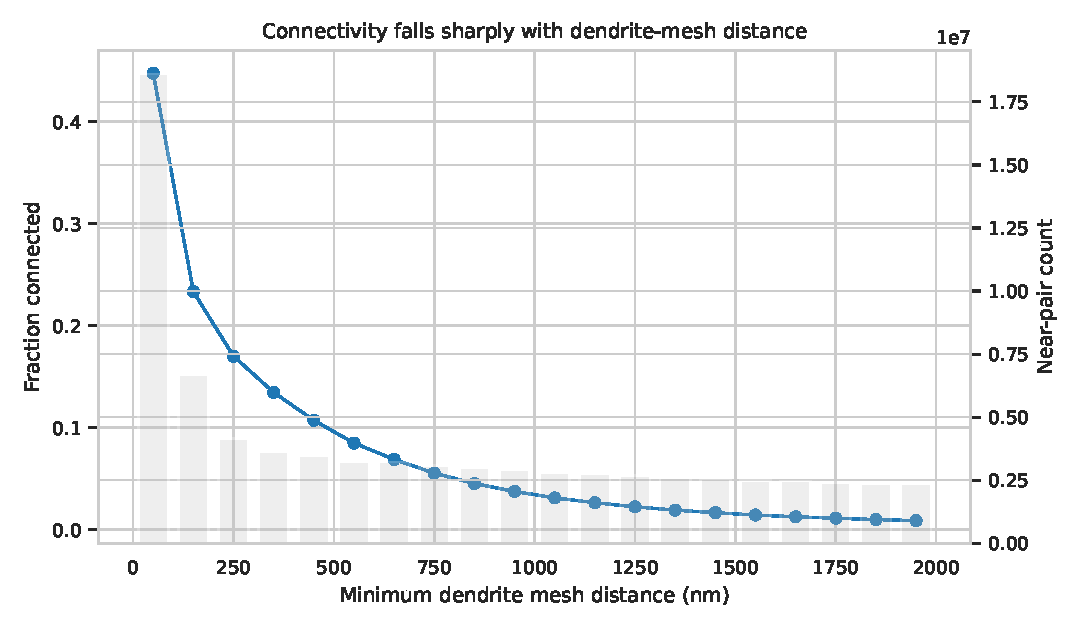
\includegraphics[width=0.88\linewidth]{figures/overall_distance_curve.pdf}
\caption{The blue line shows the observed fraction of neuron pairs with any synaptic connection in each 100 nm minimum dendrite mesh distance bin. The shaded band is the Wilson 95\% confidence interval for each bin, and the gray bars show the number of near pairs contributing to the estimate. The main quantitative takeaway is a drop from 44.7\% in the 0-100 nm bin to 0.89\% in the 1900-2000 nm bin. When bins are aggregated, the 0 to 500 nm window has fraction connected 31.3\%, whereas the 1.5 to 2.0 micron window has fraction connected 1.15\%, a 27.2 fold change.}
\label{fig:overall-distance}
\end{figure}

\begin{figure}[H]
\centering
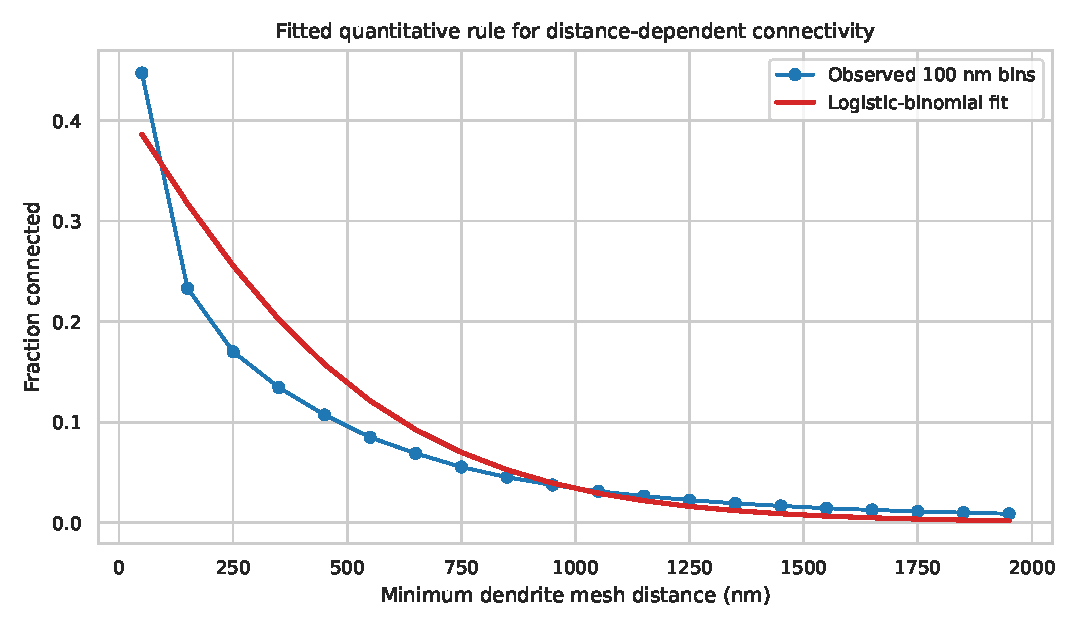
\includegraphics[width=0.88\linewidth]{figures/overall_distance_model_fit.pdf}
\caption{Points show the observed 100 nm bin fractions and the red curve shows a logistic-binomial fit to the same binned counts. This fit is used as a compact quantitative rule, not as a mechanistic model. The fitted odds ratio per additional 100 nm is 0.738, equivalent to an odds ratio of 0.048 per micron. The fitted half-rate distance is 0.37 microns, and the McFadden-style pseudo R squared is 0.219.}
\label{fig:overall-distance-model}
\end{figure}

\begin{figure}[H]
\centering
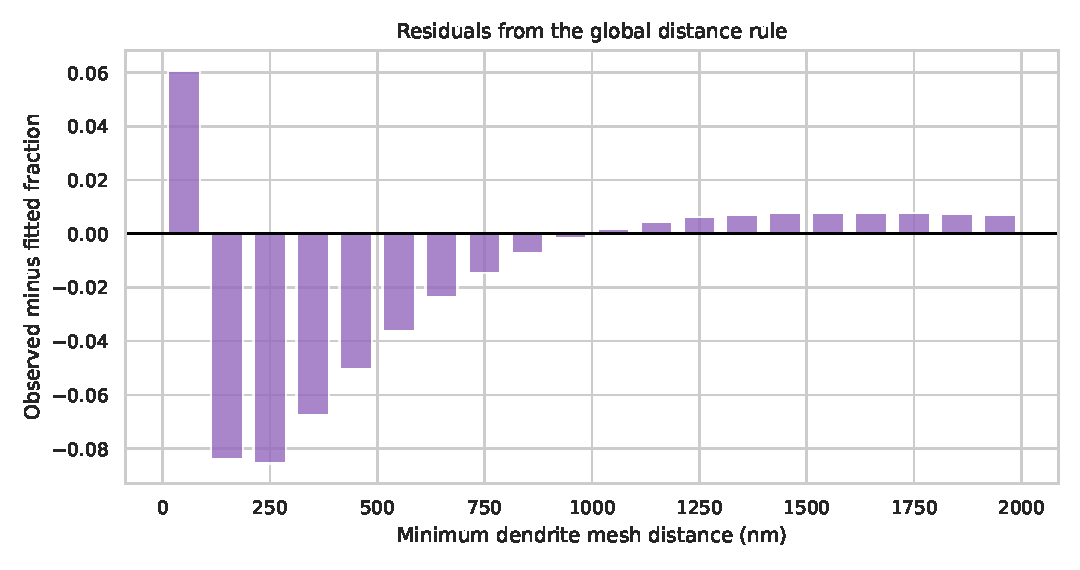
\includegraphics[width=0.88\linewidth]{figures/overall_distance_model_residuals.pdf}
\caption{Bars show observed minus fitted connection fraction for each distance bin. Positive residuals indicate bins where the global distance rule underpredicts connectivity, and negative residuals indicate overprediction. The maximum absolute residual across the 20 bins is 8.55 percentage points, which provides a scale for interpreting where the one-dimensional distance rule is insufficient.}
\label{fig:overall-distance-residuals}
\end{figure}

The fitted logistic-binomial rule estimates that each additional 100 nm multiplies connection odds by 0.738. Equivalently, each additional micron multiplies odds by 0.048. The weighted log-linear model gives a probability multiplier of 0.120 per micron and a probability half-distance of 0.33 microns. The logistic pseudo R squared is 0.219, and the weighted R squared on binned fractions is 0.920.

\subsection{Connection Strength Among Connected Pairs}

The binary connection rule asks whether a pair is connected at all. The strength analysis asks a separate question: among connected near pairs, how many synapses are present? The nearest distance bin has mean 5.38 synapses per connected pair, while the farthest bin has mean 1.67 synapses per connected pair. This comparison is conditional on being connected, so it should not be interpreted as the total expected synapse count for arbitrary near pairs.

\begin{figure}[H]
\centering
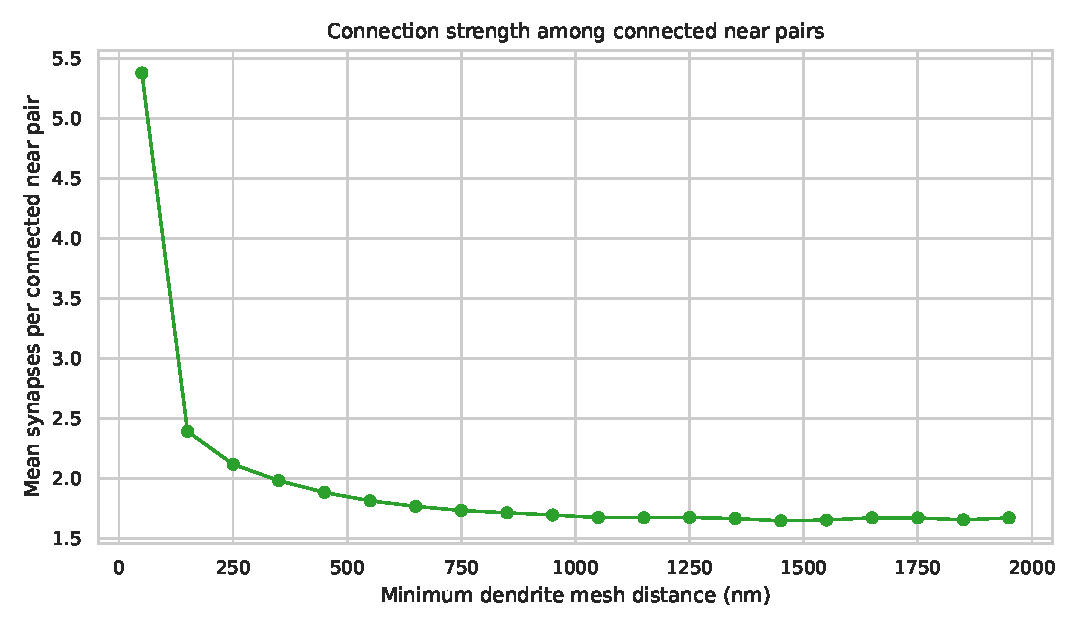
\includegraphics[width=0.88\linewidth]{figures/synapse_strength_by_distance.pdf}
\caption{The curve shows the mean total synapse count among pairs that are connected, grouped by the same 100 nm distance bins. This figure separates connection probability from connection strength among successful connections. The nearest bin has mean strength 5.38 synapses per connected pair, whereas the farthest bin has mean strength 1.67 synapses per connected pair.}
\label{fig:synapse-strength}
\end{figure}

\subsection{Broad Neuron Classes}

For broad neuron classes, the selected high-support pairs cover 77,464,215 near pairs and 12,805,154 connected pairs. The median distance-adjusted effect is log2 observed over expected 0.27, with an interquartile range of 1.03. The largest positive effect is ascending | visual\_projection, with log2 observed over expected 1.06 and fraction connected 20.0\% across 16,685 near pairs. The largest negative effect is descending | visual\_centrifugal, with log2 observed over expected -1.15 and fraction connected 7.7\% across 70,958 near pairs.

\begin{figure}[H]
\centering
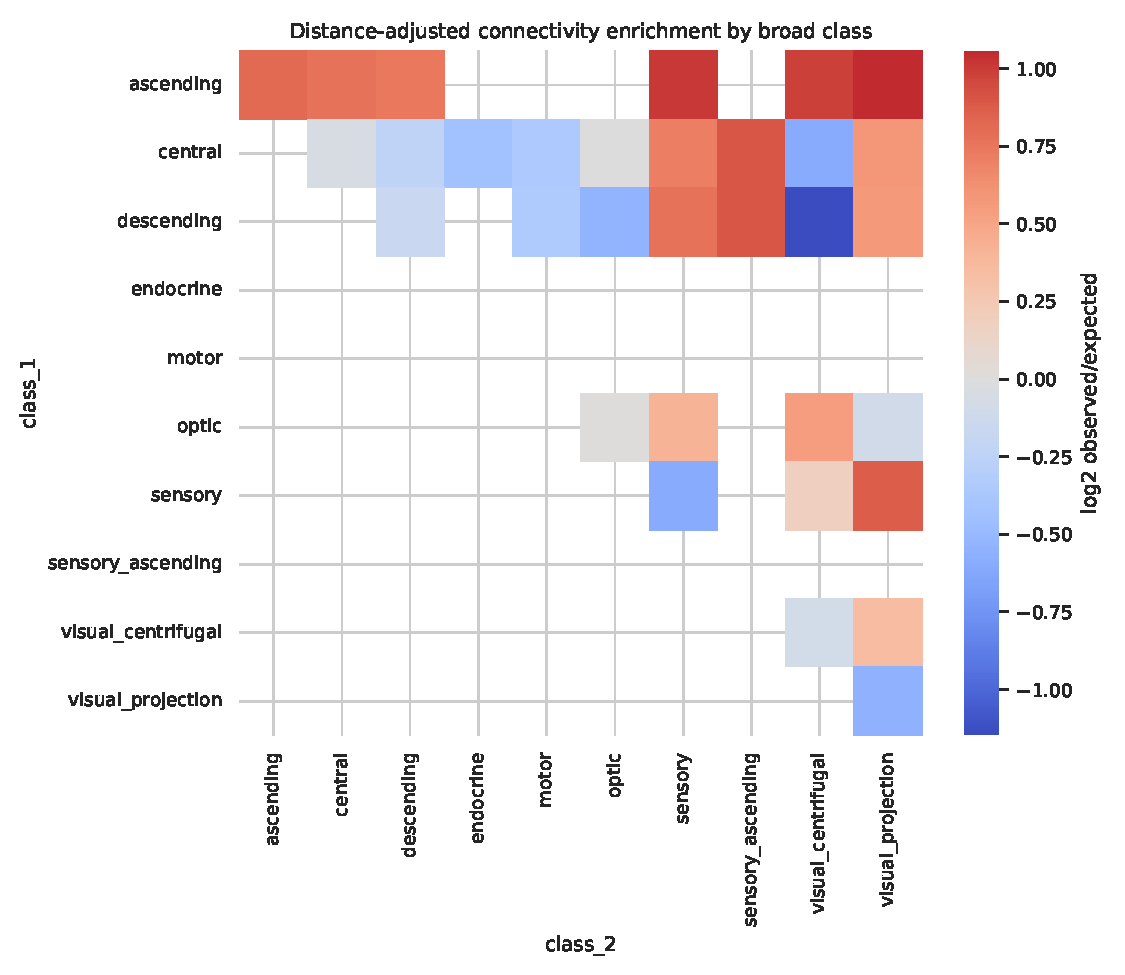
\includegraphics[width=0.82\linewidth]{figures/super_class_enrichment_heatmap.pdf}
\caption{Cells show log2 observed over expected connectivity for broad neuron class pairs after adjusting for the global distance distribution. Red values have more connected pairs than expected from distance alone, blue values have fewer, and values near zero are close to the distance-only expectation. The strongest selected broad-class enrichment is ascending | visual\_projection with log2 observed over expected 1.06.}
\label{fig:super-class-heatmap}
\end{figure}

\begin{figure}[H]
\centering
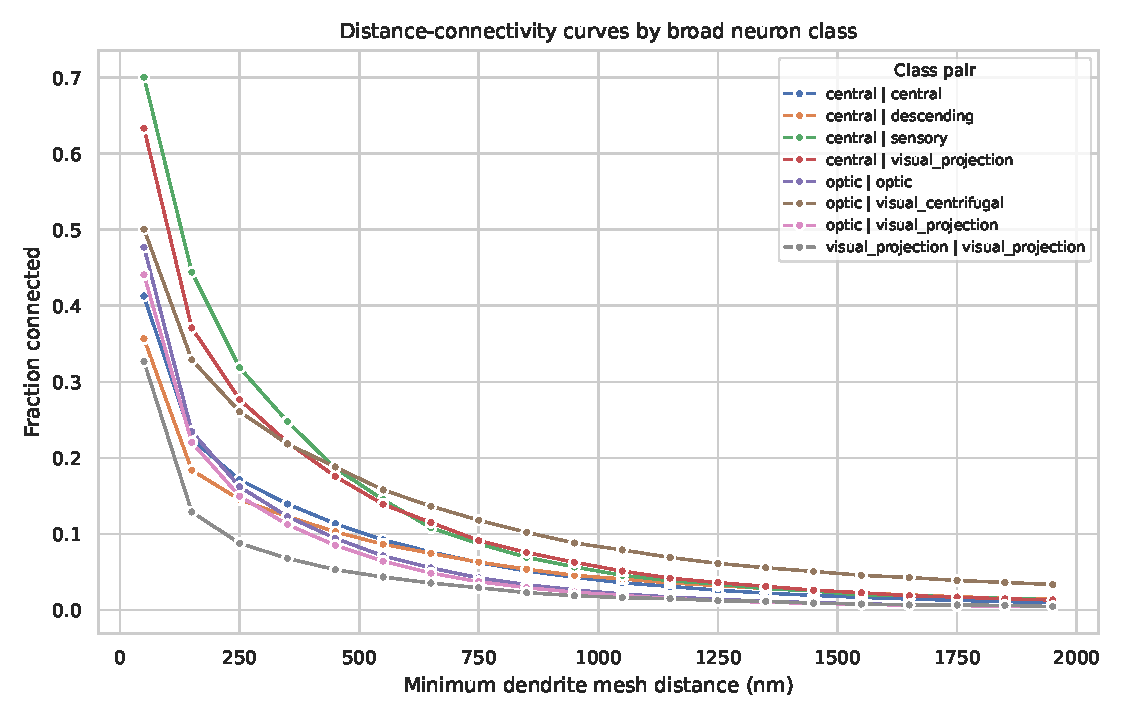
\includegraphics[width=0.88\linewidth]{figures/super_class_distance_curves.pdf}
\caption{Each line is a distance-connectivity curve for one of the highest-support broad neuron class pairs. The comparison shows that the distance rule is shared across broad classes, while the vertical separation of curves quantifies class-specific residual differences. The selected broad-class pairs cover 77,464,215 near pairs.}
\label{fig:super-class-curves}
\end{figure}

\subsection{Cell Classes and Exact Neuron Types}

For cell classes, the selected high-support pairs cover 28,581,347 near pairs and 4,899,104 connected pairs. The median distance-adjusted effect is log2 observed over expected 0.11, with an interquartile range of 1.24. The largest positive effect is LA | visual, with log2 observed over expected 1.53 and fraction connected 32.5\% across 13,972 near pairs. The largest negative effect is LO>LOP | ME>LOP.LO, with log2 observed over expected -2.64 and fraction connected 1.1\% across 8,486 near pairs.

For exact neuron types, the selected high-support pairs cover 4,948,340 near pairs and 569,600 connected pairs. The median distance-adjusted effect is log2 observed over expected -0.60, with an interquartile range of 4.66. The largest positive effect is T2 | cL21, with log2 observed over expected 2.14 and fraction connected 97.5\% across 2,776 near pairs. The largest negative effect is Lawf2 | Tm9, with log2 observed over expected -5.29 and fraction connected 0.3\% across 6,827 near pairs.

\begin{figure}[H]
\centering
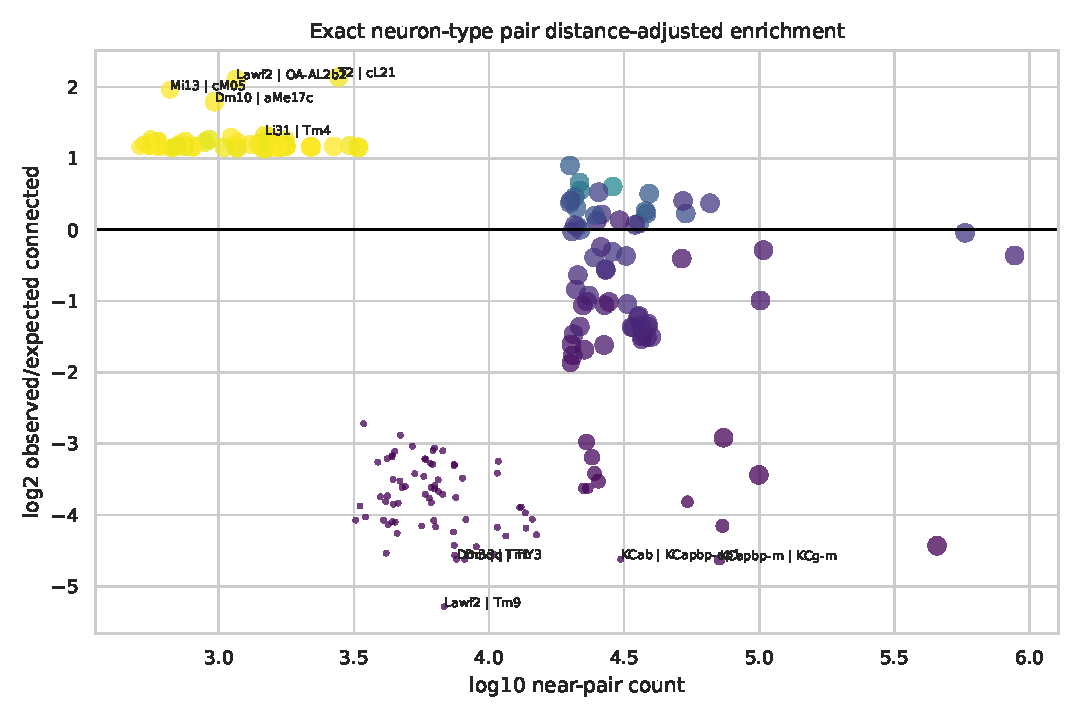
\includegraphics[width=0.88\linewidth]{figures/cell_type_enrichment_scatter.pdf}
\caption{Each point is a selected exact neuron-type pair. The x-axis is log10 near-pair support, the y-axis is distance-adjusted log2 observed over expected connectivity, point color is raw fraction connected, and point area increases with connected-pair count. This representation distinguishes high-confidence effects from small-support outliers. The strongest selected exact-type enrichment is T2 | cL21, with log2 observed over expected 2.14.}
\label{fig:cell-type-scatter}
\end{figure}

\subsection{Brain Regions}

For dominant postsynaptic neuropils, the selected high-support pairs cover 59,918,001 near pairs and 10,241,532 connected pairs. The median distance-adjusted effect is log2 observed over expected -0.06, with an interquartile range of 1.06. The largest positive effect is LOP\_L | LOP\_R, with log2 observed over expected 1.56 and fraction connected 33.1\% across 6,906 near pairs. The largest negative effect is AVLP\_L | MB\_CA\_L, with log2 observed over expected -2.43 and fraction connected 0.4\% across 8,809 near pairs.

For dominant presynaptic neuropils, the selected high-support pairs cover 54,670,227 near pairs and 9,602,716 connected pairs. The median distance-adjusted effect is log2 observed over expected -0.04, with an interquartile range of 1.72. The largest positive effect is MB\_CA\_R | MB\_ML\_R, with log2 observed over expected 0.99 and fraction connected 34.3\% across 19,166 near pairs. The largest negative effect is IB\_L | MB\_ML\_L, with log2 observed over expected -4.11 and fraction connected 0.4\% across 2,239 near pairs.

\begin{figure}[H]
\centering
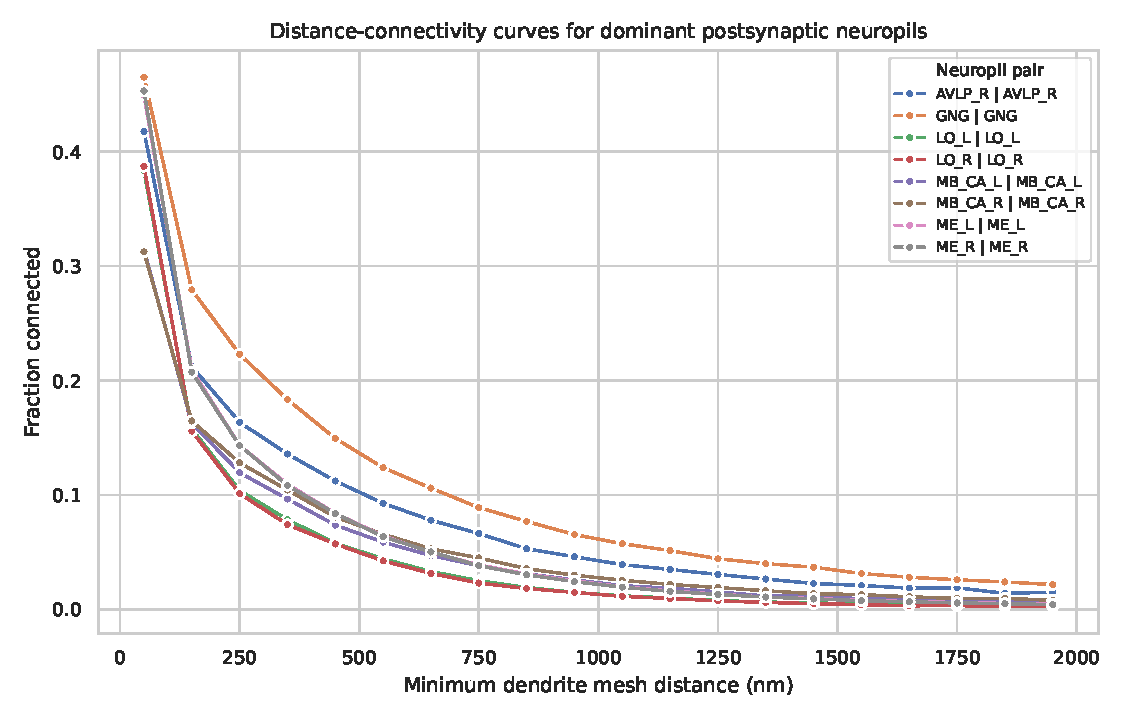
\includegraphics[width=0.9\linewidth]{figures/post_neuropil_distance_curves.pdf}
\caption{Lines show distance-connectivity curves for high-support same-region pairs defined by dominant postsynaptic neuropil. Each point is a 100 nm bin fraction, so differences between curves indicate region-specific connectivity beyond the global distance trend. The selected postsynaptic neuropil pairs cover 59,918,001 near pairs.}
\label{fig:post-neuropil-curves}
\end{figure}

\begin{figure}[H]
\centering
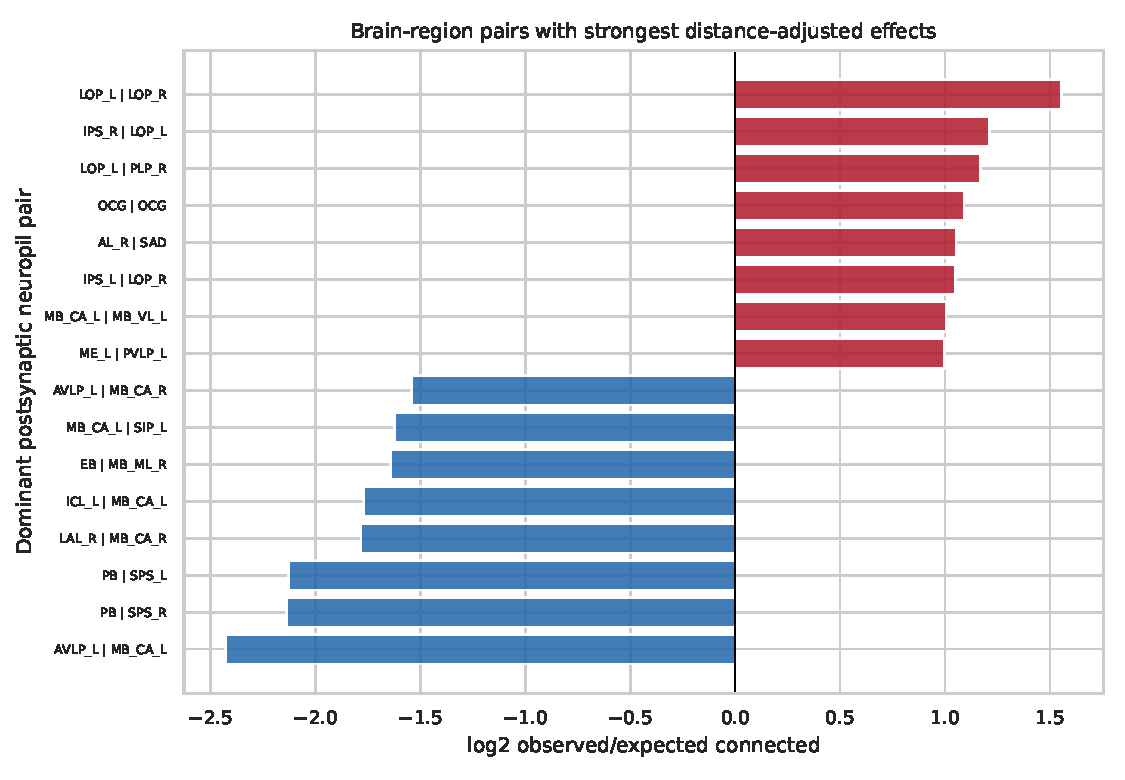
\includegraphics[width=0.9\linewidth]{figures/post_neuropil_enrichment_extremes.pdf}
\caption{Bars show the largest positive and negative distance-adjusted effects for dominant postsynaptic neuropil pairs. Positive bars are pairs with more connected pairs than predicted by distance composition, and negative bars are pairs with fewer. The top enriched selected region pair is LOP\_L | LOP\_R, with log2 observed over expected 1.56. The strongest depletion is AVLP\_L | MB\_CA\_L, with log2 observed over expected -2.43.}
\label{fig:post-neuropil-extremes}
\end{figure}

\subsection{Neurotransmitter, Flow, and Side}

For canonical neurotransmitter pairs, the selected high-support pairs cover 77,498,792 near pairs and 12,811,761 connected pairs. The median distance-adjusted effect is log2 observed over expected -0.00, with an interquartile range of 0.22. The largest positive effect is gaba | serotonin, with log2 observed over expected 0.25 and fraction connected 17.0\% across 165,608 near pairs. The largest negative effect is octopamine | octopamine, with log2 observed over expected -0.98 and fraction connected 16.8\% across 1,091 near pairs.

For flow labels, the selected high-support pairs cover 77,514,353 near pairs and 12,812,504 connected pairs. The median distance-adjusted effect is log2 observed over expected 0.01, with an interquartile range of 0.69. The largest positive effect is afferent | efferent, with log2 observed over expected 0.75 and fraction connected 20.8\% across 322,683 near pairs. The largest negative effect is efferent | intrinsic, with log2 observed over expected -0.23 and fraction connected 14.6\% across 2,146,760 near pairs.

For hemisphere side labels, the selected high-support pairs cover 77,514,283 near pairs and 12,812,503 connected pairs. The median distance-adjusted effect is log2 observed over expected 0.20, with an interquartile range of 0.36. The largest positive effect is na | right, with log2 observed over expected 0.42 and fraction connected 18.3\% across 2,702 near pairs. The largest negative effect is left | left, with log2 observed over expected -0.05 and fraction connected 16.1\% across 34,000,292 near pairs.

\begin{figure}[H]
\centering
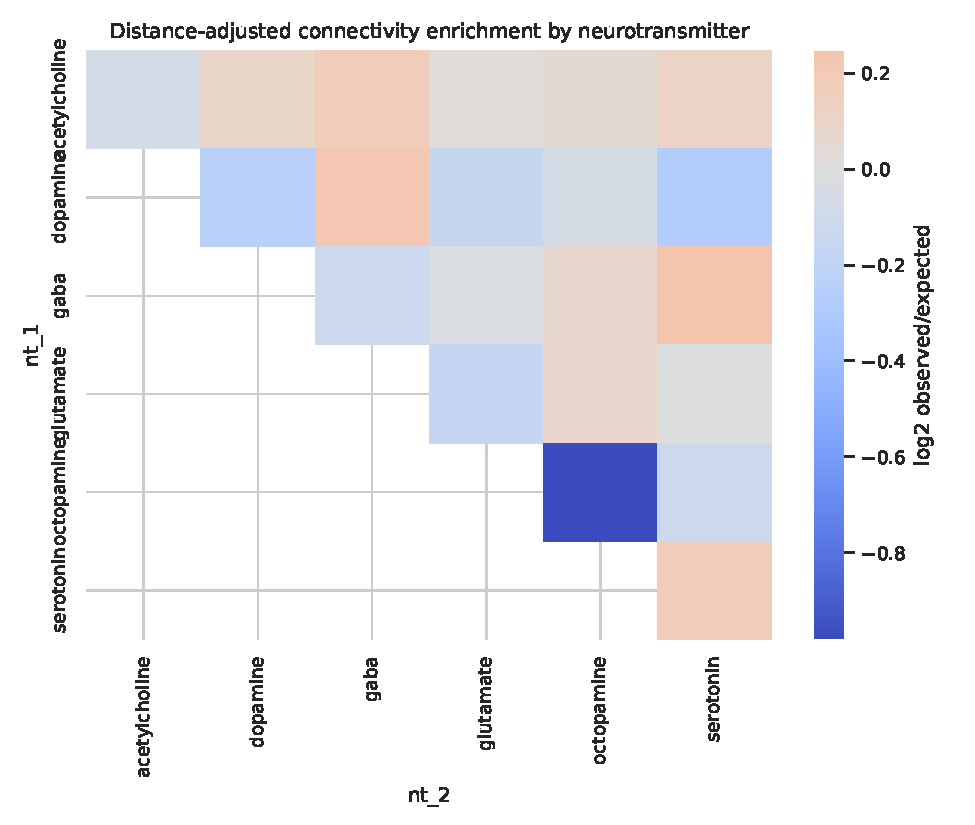
\includegraphics[width=0.78\linewidth]{figures/nt_enrichment_heatmap.pdf}
\caption{Cells show the same distance-adjusted observed over expected statistic after grouping each pair by canonical neurotransmitter labels. The narrower color range relative to some anatomical partitions means that broad neurotransmitter identity explains less residual variation after distance adjustment. The strongest selected neurotransmitter enrichment is gaba | serotonin, with log2 observed over expected 0.25.}
\label{fig:nt-heatmap}
\end{figure}

\begin{figure}[H]
\centering
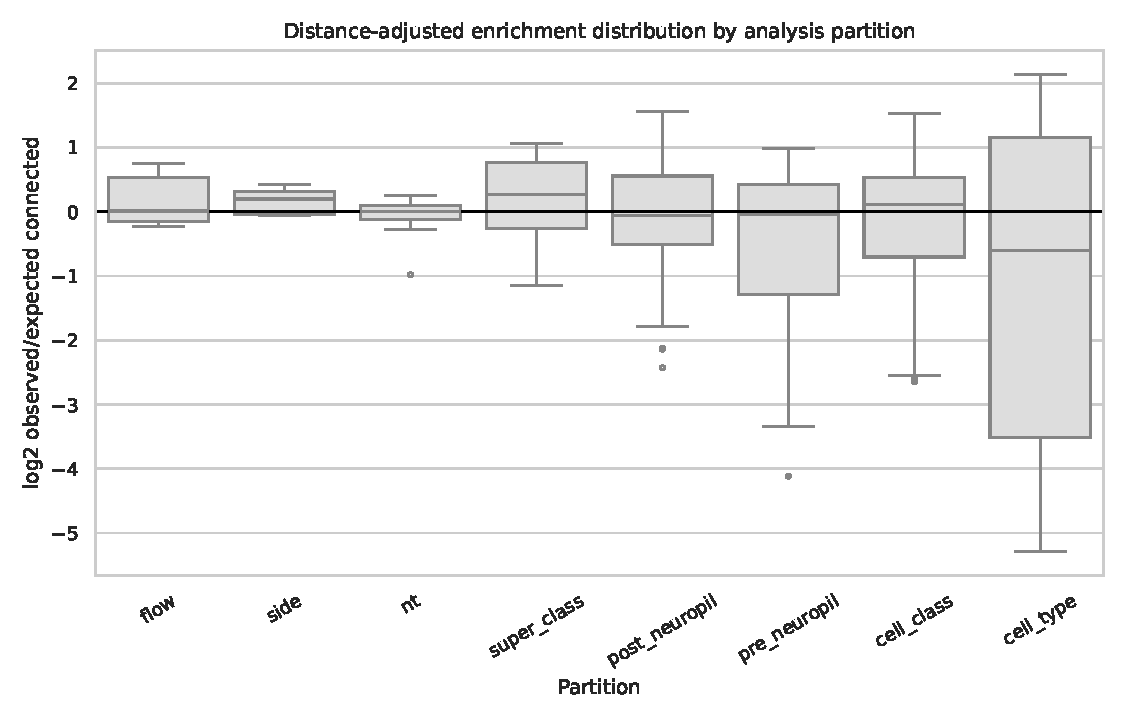
\includegraphics[width=0.88\linewidth]{figures/partition_enrichment_summary.pdf}
\caption{Boxes summarize the distribution of distance-adjusted log2 observed over expected effects among selected high-support pairs for each partition. The zero line is the distance-only expectation. Wider boxes and longer tails identify partitions where metadata labels capture more residual structure after controlling for distance. In this selected set, exact neuron type spans from -5.29 to 2.14 in log2 observed over expected.}
\label{fig:partition-summary}
\end{figure}

\subsection{Distance-Adjusted Effect Tables}

\begin{table}[htbp]
\centering
\small
\caption{Broad neuron class pairs with the largest positive and negative distance-adjusted effects among selected supported pairs.}
\label{tab:super-class-extremes}
\resizebox{\linewidth}{!}{%
\begin{tabular}{llrrrrr}
\toprule
Direction & Pair & Near pairs & Connected & Fraction & Expected & log$_2$(O/E) \\
\midrule
enriched & ascending | visual\_projection & 16,685 & 3,343 & 0.200 & 1605.1 & 1.06 \\
enriched & ascending | sensory & 81,435 & 21,991 & 0.270 & 10899.0 & 1.01 \\
enriched & ascending | visual\_centrifugal & 19,359 & 3,953 & 0.204 & 1999.1 & 0.98 \\
enriched & central | sensory\_ascending & 46,781 & 7,542 & 0.161 & 4040.1 & 0.90 \\
enriched & descending | sensory\_ascending & 11,373 & 1,611 & 0.142 & 864.2 & 0.90 \\
depleted & descending | visual\_centrifugal & 70,958 & 5,460 & 0.077 & 12100.1 & -1.15 \\
depleted & sensory | sensory & 282,980 & 28,073 & 0.099 & 42671.1 & -0.60 \\
depleted & central | visual\_centrifugal & 691,153 & 71,926 & 0.104 & 108960.8 & -0.60 \\
depleted & visual\_projection | visual\_projection & 2,006,829 & 290,967 & 0.145 & 429035.9 & -0.56 \\
depleted & descending | optic & 67,108 & 4,619 & 0.069 & 6709.4 & -0.54 \\
\bottomrule
\end{tabular}
}
\end{table}

\begin{table}[htbp]
\centering
\small
\caption{Cell class pairs with the largest positive and negative distance-adjusted effects among selected supported pairs.}
\label{tab:cell-class-extremes}
\resizebox{\linewidth}{!}{%
\begin{tabular}{llrrrrr}
\toprule
Direction & Pair & Near pairs & Connected & Fraction & Expected & log$_2$(O/E) \\
\midrule
enriched & LA | visual & 13,972 & 4,539 & 0.325 & 1573.6 & 1.53 \\
enriched & Kenyon\_Cell | MBIN & 10,691 & 10,399 & 0.973 & 4658.9 & 1.16 \\
enriched & LA>ME | visual & 79,522 & 24,975 & 0.314 & 11726.6 & 1.09 \\
enriched & AN | mechanosensory & 72,955 & 20,489 & 0.281 & 10020.6 & 1.03 \\
enriched & Kenyon\_Cell | MBON & 121,933 & 62,664 & 0.514 & 31450.1 & 0.99 \\
depleted & LO>LOP | ME>LOP.LO & 8,486 & 95 & 0.011 & 594.5 & -2.64 \\
depleted & ME>LO.LOP | visual & 40,829 & 233 & 0.006 & 1402.9 & -2.59 \\
depleted & ME>LOP | ME>LOP.LO & 6,515 & 67 & 0.010 & 395.5 & -2.55 \\
depleted & ME>LOP.LO | visual & 5,721 & 67 & 0.012 & 337.1 & -2.32 \\
depleted & ME>LA | ME>LO.LOP & 240,838 & 8,228 & 0.034 & 35133.1 & -2.09 \\
\bottomrule
\end{tabular}
}
\end{table}

\begin{table}[htbp]
\centering
\small
\caption{Dominant postsynaptic neuropil pairs with the largest positive and negative distance-adjusted effects among selected supported pairs.}
\label{tab:post-neuropil-extremes}
\resizebox{\linewidth}{!}{%
\begin{tabular}{llrrrrr}
\toprule
Direction & Pair & Near pairs & Connected & Fraction & Expected & log$_2$(O/E) \\
\midrule
enriched & LOP\_L | LOP\_R & 6,906 & 2,287 & 0.331 & 777.5 & 1.56 \\
enriched & IPS\_R | LOP\_L & 5,316 & 1,643 & 0.309 & 708.2 & 1.21 \\
enriched & LOP\_L | PLP\_R & 2,927 & 805 & 0.275 & 357.5 & 1.17 \\
enriched & OCG | OCG & 4,033 & 1,334 & 0.331 & 626.2 & 1.09 \\
enriched & AL\_R | SAD & 2,909 & 807 & 0.277 & 388.8 & 1.05 \\
depleted & AVLP\_L | MB\_CA\_L & 8,809 & 39 & 0.004 & 212.0 & -2.43 \\
depleted & PB | SPS\_R & 3,685 & 71 & 0.019 & 314.0 & -2.14 \\
depleted & PB | SPS\_L & 3,660 & 66 & 0.018 & 290.4 & -2.13 \\
depleted & LAL\_R | MB\_CA\_R & 4,110 & 32 & 0.008 & 111.3 & -1.78 \\
depleted & ICL\_L | MB\_CA\_L & 5,048 & 38 & 0.008 & 130.8 & -1.77 \\
\bottomrule
\end{tabular}
}
\end{table}

\begin{table}[htbp]
\centering
\small
\caption{Dominant presynaptic neuropil pairs with the largest positive and negative distance-adjusted effects among selected supported pairs.}
\label{tab:pre-neuropil-extremes}
\resizebox{\linewidth}{!}{%
\begin{tabular}{llrrrrr}
\toprule
Direction & Pair & Near pairs & Connected & Fraction & Expected & log$_2$(O/E) \\
\midrule
enriched & MB\_CA\_R | MB\_ML\_R & 19,166 & 6,568 & 0.343 & 3315.2 & 0.99 \\
enriched & LA\_L | LA\_L & 25,255 & 6,794 & 0.269 & 3470.0 & 0.97 \\
enriched & AL\_R | MB\_CA\_R & 4,132 & 1,972 & 0.477 & 1048.8 & 0.91 \\
enriched & AL\_L | MB\_CA\_L & 4,397 & 2,001 & 0.455 & 1065.8 & 0.91 \\
enriched & PB | PB & 3,568 & 1,713 & 0.480 & 913.2 & 0.91 \\
depleted & IB\_L | MB\_ML\_L & 2,239 & 8 & 0.004 & 146.7 & -4.11 \\
depleted & ATL\_L | MB\_ML\_L & 2,808 & 18 & 0.006 & 187.6 & -3.35 \\
depleted & ICL\_R | MB\_ML\_R & 8,450 & 30 & 0.004 & 287.4 & -3.24 \\
depleted & LA\_L | LOP\_L & 3,806 & 52 & 0.014 & 381.7 & -2.86 \\
depleted & LA\_R | LOP\_R & 8,318 & 135 & 0.016 & 932.3 & -2.78 \\
\bottomrule
\end{tabular}
}
\end{table}

\begin{table}[htbp]
\centering
\small
\caption{Neurotransmitter pairs with the largest positive and negative distance-adjusted effects among selected supported pairs.}
\label{tab:nt-extremes}
\resizebox{\linewidth}{!}{%
\begin{tabular}{llrrrrr}
\toprule
Direction & Pair & Near pairs & Connected & Fraction & Expected & log$_2$(O/E) \\
\midrule
enriched & gaba | serotonin & 165,608 & 28,181 & 0.170 & 23739.6 & 0.25 \\
enriched & dopamine | gaba & 381,423 & 71,731 & 0.188 & 61267.7 & 0.23 \\
enriched & serotonin | serotonin & 50,397 & 10,500 & 0.208 & 9299.7 & 0.18 \\
enriched & acetylcholine | gaba & 15,613,124 & 3,099,439 & 0.199 & 2762765.2 & 0.17 \\
enriched & acetylcholine | serotonin & 613,820 & 93,718 & 0.153 & 86533.0 & 0.12 \\
depleted & octopamine | octopamine & 1,091 & 183 & 0.168 & 361.6 & -0.98 \\
depleted & dopamine | serotonin & 35,033 & 3,474 & 0.099 & 4197.5 & -0.27 \\
depleted & dopamine | dopamine & 3,193,624 & 358,505 & 0.112 & 424314.7 & -0.24 \\
depleted & glutamate | glutamate & 3,827,209 & 578,349 & 0.151 & 647850.8 & -0.16 \\
depleted & dopamine | glutamate & 622,380 & 77,558 & 0.125 & 86487.2 & -0.16 \\
\bottomrule
\end{tabular}
}
\end{table}

\begin{table}[htbp]
\centering
\small
\caption{Exact neuron type pairs with the largest positive and negative distance-adjusted effects among selected supported pairs.}
\label{tab:cell-type-extremes}
\resizebox{\linewidth}{!}{%
\begin{tabular}{llrrrrr}
\toprule
Direction & Pair & Near pairs & Connected & Fraction & Expected & log$_2$(O/E) \\
\midrule
enriched & T2 | cL21 & 2,776 & 2,706 & 0.975 & 614.7 & 2.14 \\
enriched & Lawf2 | OA-AL2b2 & 1,160 & 1,150 & 0.991 & 267.1 & 2.10 \\
enriched & Mi13 | cM05 & 660 & 659 & 0.998 & 169.1 & 1.96 \\
enriched & Dm10 | aMe17c & 965 & 954 & 0.989 & 275.3 & 1.79 \\
enriched & Li31 | Tm4 & 1,480 & 1,449 & 0.979 & 580.1 & 1.32 \\
depleted & Lawf2 | Tm9 & 6,827 & 21 & 0.003 & 838.9 & -5.29 \\
depleted & KCapbp-m | KCg-m & 71,290 & 257 & 0.004 & 6368.6 & -4.63 \\
depleted & Dm3q | T1 & 8,134 & 20 & 0.002 & 505.1 & -4.62 \\
depleted & KCab | KCapbp-ap1 & 30,706 & 84 & 0.003 & 2082.0 & -4.62 \\
depleted & Dm3q | TmY3 & 7,588 & 20 & 0.003 & 504.6 & -4.62 \\
\bottomrule
\end{tabular}
}
\end{table}

\begin{table}[htbp]
\centering
\small
\caption{Flow pairs with the largest positive and negative distance-adjusted effects among selected supported pairs.}
\label{tab:flow-extremes}
\resizebox{\linewidth}{!}{%
\begin{tabular}{llrrrrr}
\toprule
Direction & Pair & Near pairs & Connected & Fraction & Expected & log$_2$(O/E) \\
\midrule
enriched & afferent | efferent & 322,683 & 67,261 & 0.208 & 39974.4 & 0.75 \\
enriched & afferent | intrinsic & 2,271,556 & 426,365 & 0.188 & 263327.5 & 0.70 \\
enriched & afferent | afferent & 429,667 & 62,545 & 0.146 & 60821.0 & 0.04 \\
enriched & intrinsic | intrinsic & 72,131,799 & 11,906,258 & 0.165 & 12038589.3 & -0.02 \\
enriched & efferent | efferent & 211,888 & 37,440 & 0.177 & 43177.7 & -0.21 \\
depleted & efferent | intrinsic & 2,146,760 & 312,635 & 0.146 & 366243.4 & -0.23 \\
depleted & efferent | efferent & 211,888 & 37,440 & 0.177 & 43177.7 & -0.21 \\
depleted & intrinsic | intrinsic & 72,131,799 & 11,906,258 & 0.165 & 12038589.3 & -0.02 \\
depleted & afferent | afferent & 429,667 & 62,545 & 0.146 & 60821.0 & 0.04 \\
depleted & afferent | intrinsic & 2,271,556 & 426,365 & 0.188 & 263327.5 & 0.70 \\
\bottomrule
\end{tabular}
}
\end{table}

\begin{table}[htbp]
\centering
\small
\caption{Side pairs with the largest positive and negative distance-adjusted effects among selected supported pairs.}
\label{tab:side-extremes}
\resizebox{\linewidth}{!}{%
\begin{tabular}{llrrrrr}
\toprule
Direction & Pair & Near pairs & Connected & Fraction & Expected & log$_2$(O/E) \\
\midrule
enriched & na | right & 2,702 & 494 & 0.183 & 368.4 & 0.42 \\
enriched & left | right & 7,951,633 & 1,472,387 & 0.185 & 1108888.6 & 0.41 \\
enriched & left | na & 2,792 & 467 & 0.167 & 382.6 & 0.29 \\
enriched & center | left & 157,811 & 31,235 & 0.198 & 27022.9 & 0.21 \\
enriched & center | right & 160,597 & 31,292 & 0.195 & 27428.8 & 0.19 \\
depleted & left | left & 34,000,292 & 5,462,670 & 0.161 & 5658493.1 & -0.05 \\
depleted & right | right & 35,235,592 & 5,813,227 & 0.165 & 5988787.9 & -0.04 \\
depleted & center | center & 2,864 & 731 & 0.255 & 753.0 & -0.04 \\
depleted & center | right & 160,597 & 31,292 & 0.195 & 27428.8 & 0.19 \\
depleted & center | left & 157,811 & 31,235 & 0.198 & 27022.9 & 0.21 \\
\bottomrule
\end{tabular}
}
\end{table}

\section{Discussion}

The most defensible quantitative rule from this analysis is that dendrite mesh proximity is a powerful but incomplete predictor of synaptic connectivity. The evidence for the rule is the monotonic decline from 44.7\% in the nearest bin to 0.89\% in the farthest bin, the 27.2 fold contrast between the close and far aggregate windows, and the fitted odds multiplier per 100 nm. The residual and partition analyses show that distance does not explain all structure.

The distance-adjusted enrichments identify metadata partitions whose labels preserve residual connectivity structure after controlling for the global distance distribution. Exact neuron type and brain-region labels show the widest selected effects, which is expected if cell identity and regional circuit architecture impose specific partner preferences beyond physical opportunity. Neurotransmitter labels show smaller selected effects, which is consistent with neurotransmitter being a broad physiological class rather than a precise partner-identity label.

A practical rule for downstream analysis is to treat 0 to 500 nm as a high-opportunity zone and 1.5 to 2.0 microns as a low-opportunity zone under this mesh sampling definition. The high-opportunity zone is connected at 31.3\%, while the low-opportunity zone is connected at 1.15\%. This does not mean distance alone should be used as a classifier. Instead, it provides a baseline expectation against which region, cell type, neurotransmitter, flow, and side effects can be evaluated.

\section{Limitations}

The mesh-distance variable is computed from sampled vertices near postsynaptic sites, not from a complete continuous surface-to-surface distance between all dendritic compartments. The 250 nm sampling interval and 500 nm postsynaptic-site radius make the computation tractable at whole-brain scale, but they also define the resolution and biological interpretation of the distance measure.

The report uses the binary question of whether any synaptic connection exists between a near pair. Direction, synapse count, and sign are retained in the enriched table and in the strength summaries, but most partition effects use the binary connected-any outcome. Exact neuron-type plots are selected for support and effect visibility, so the figure is an interpretable high-support view rather than a complete plot of every type pair.

The observed over expected adjustment controls for the global distance-bin distribution but does not control simultaneously for every possible confounder, such as neuron size, synapse count, sampling density, or nested cell-type structure. Claims in this report should therefore be read as descriptive whole-connectome statistics and as hypothesis-generating evidence for circuit specificity.

\section{Reproducibility and Outputs}

The full enriched near-pair table is stored as \texttt{near\_pairs\_enriched.parquet} in the canonical run directory. The report directory contains the compiled PDF, LaTeX source, figure PDFs, CSV tables, and a JSON manifest with all headline metrics. Lightweight CSV tables are suitable for versioned snapshots. Bulk Parquet tables and mesh caches are intentionally excluded from the repository snapshot.

\end{document}
